\documentclass[12pt]{report}
\usepackage[english]{babel}
\usepackage[utf8]{inputenc}
\usepackage{array}
\usepackage{authblk}
\usepackage{appendix}
\usepackage{booktabs}
\usepackage{float}
\usepackage{gensymb}
\usepackage{graphicx}
\usepackage[implicit=false]{hyperref}
\usepackage{listings}
\usepackage{minted}
\usepackage{multirow}
\usepackage{natbib}
\usepackage{ragged2e}

\usepackage{geometry}
 \geometry{
 a4paper,
 total={170mm,257mm},
 left=20mm,
 top=20mm,
 }
 
 \hypersetup{
    colorlinks=true,
    linkcolor=blue,
    filecolor=magenta,      
    urlcolor=cyan,
}

%\title{Autonomous Robotic Mapping and Navigation}
%\author{Armanda, Chris Benhard; Barakat, Housam; Veloso, Michael}
%\affil[]{RMIT University}
%\date{October 2018}

\begin{document}

\begin{titlepage}
\newcommand{\HRule}{\rule{\linewidth}{0.5mm}} % Defines a new command for the horizontal lines, change thickness here

\center % Center everything on the page
 
%----------------------------------------------------------------------------------------
%	HEADING SECTIONS
%----------------------------------------------------------------------------------------

\textsc{\LARGE RMIT University}\\[1.5cm] % Name of your university/college
\textsc{\Large Final Report}\\[0.5cm] % Major heading such as course name
\textsc{\large In fulfilment of OENG1168 Engineering Capstone Project 4B}\\[0.5cm] % Minor heading such as course title

%----------------------------------------------------------------------------------------
%	TITLE SECTION
%----------------------------------------------------------------------------------------

\HRule \\[0.4cm]
{ \huge \bfseries Autonomous Robotic Mapping and Navigation}\\[0.25cm] % Title of your document
\HRule \\[1.25cm]
 
%----------------------------------------------------------------------------------------
%	AUTHOR SECTION
%----------------------------------------------------------------------------------------

\begin{minipage}{0.4\textwidth}
\begin{flushleft} \large
\emph{Author:}\\
Chris Benhard \textsc{Armanda} (s3626565)\\ % Your name
Housam \textsc{Barakat} (s3401160)\\
Michael \textsc{Veloso} (s3485068)
\end{flushleft}
\end{minipage}
~
\begin{minipage}{0.4\textwidth}
\begin{flushright} \large
\emph{Supervisor:} \\
Dr. Akram \textsc{Hourani}\\
\textsc{ } \\
\textsc{ } % Supervisor's Name
 
\end{flushright}
\end{minipage}\\[1cm]

\end{titlepage}

%\maketitle

\chapter*{Abstract}

Autonomous navigation and mapping is starting to be more well known as it can be used in a variety of applications. From being deployed to search and rescue missions, exploration, disaster zones and picking and storage as well. In this report, the above mentioned applications will be presented and the related software to allow the robots to possess such skills. The algorithms Hector\_SLAM and Gmapping will be compared, in terms of localization and mapping capabilities in an urban environment. All software used has been used internationally, for many purposes. As of the current date, Autonomous Mapping and Navigation has been researched further for the main purpose of search and rescue.\par

\tableofcontents
\newpage
\listoffigures

\chapter{Introduction}
The concept of Autonomous Mapping and Navigation is becoming increasingly popular in the recent years, thanks to smart cars manufacturers, the most well known being Tesla. The concept however is no longer exclusively useful only to build smart cars, but also have been introduced to robots to do seemingly menial tasks to increase work efficiency and at the same time to decrease costs and manpower. Amazon, the online retail giant, is known to have several robots equipped with autonomous mapping and navigation in their warehouses to keep accurate inventory without the need of a employing large number of warehouse workers.\par
\vspace{1em}
Although robot with self-localization and mapping (SLAM) offers many benefits, they are usually expensive for personal use. Such robots are also usually fit for single purpose. This project aims to offer a cheaper option of SLAM robots that is both fully configurable and open-sourced. TurtleBot3 has been decided to be procured for the purpose of this project, since its documentation is comprehensive and supported by the growing community, helping to build variations of the robot to execute more than one purpose. The robot was preloaded and programmed with Robot Operating System (ROS), a pseudo-operating system residing side-by-side with a functioning Linux Ubuntu system.\par
\chapter{Statement of Problem}
By aiming for fully autonomous mapping and navigation there are multiple applications that we can reach out to. Most notable fields are:\par
\begin{itemize}
    \item \textbf{Exploration}\par
    Which can now be done autonomously, by sending in a configured robot this will allow it to fully traverse the terrain without being hindered by any obstacle while simultaneously mapping the surroundings and transmitting the data to a remote laptop. One of the huge advantages of using autonomous robots in such a dangerous field, is the lowering of the mortality rate. These robots can be deployed in an urban search and rescue mission, deployed in disaster zones and other such related areas. Robots are expendable, can be fully configured and prepared for most scenarios, making it much more easier and safer. Humans on the other hand are not expendable, it takes time to train, money to prepare and procedures that they need to remember for every situation. Even when a fully trained human is been given the proper gear and instructions which will leave them ready to face most scenarios, there will always still be a mortality rate present due to the nature of their profession. To effectively lower the mortality rate in this particular field, autonomous robotics would be the ideal tool.\par
    \begin{figure}[H]
        \centering
        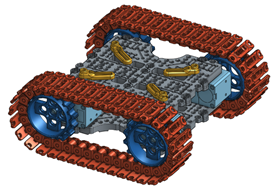
\includegraphics{Fig1.png}
        \caption{Unique all-terrain robotic solution}
        \label{fig:1}
    \end{figure}


    \item \textbf{Picking and Storage}\par
    Automated picking of components and storing them in predetermined locations is another area we can branch out to as well. Utilising a robotic arm with sensors allows the robot to detect the type of component,size and then map a path towards the storage location. Having a automated storage also ensures that the system being used can keep track of every delivery therefore reducing any downtime. Automating a picking and storage system can create big leaps in terms of efficiency and lean manufacturing.\par
    \begin{figure}[H]
        \centering
        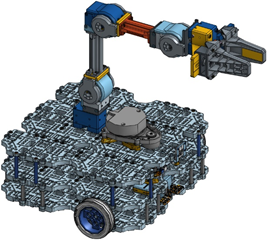
\includegraphics{Fig2.png}
        \caption{Unique picking and storing solution}
        \label{fig:2}
    \end{figure}
    
    \item \textbf{Emergency Relief}\par
    Fitting the TurtleBot3 with a fire resistant exterior, will allow the robot to go into buildings with low structural integrity or any environments deemed to dangerous for humans and map the location. Fully configured with the proper hardware will allow the robot to locate sources of extreme heat and be able to tell the different heat temperatures so civilians in distress can be identified. By having the assistance of a autonomous robot Firefighters will be able to locate civilians much faster and more efficiently, theoretically removing the amount of time spent in a dangerous environment and the amount of casualties usually associated with the job. (current work in progress)\par
    
\end{itemize}
\chapter{Literature Review}
SLAM Robots in the past have been involved in high-profile operations, including the 9/11 disaster \cite{Liu}. Such robots have proved beneficial during SAR operations, as disaster areas may still be lethally dangerous for human due to collapsing building structure or poisonous air, and psychologically demanding. Hence robots are seen as an alternative method to reach such areas thought unsafe for professional SAR teams to do so \cite{Murphy}. It is generally accepted that a certain degree of self autonomy should be assigned to robots in scenarios where time and speed are crucial. However, there is no consensus whether a robot should be given full autonomy or should it be supervised by a human controller who is able to override the robot’s decisions. although Robot Operating System (ROS) has provided methods for both options, deciding which to choose is still considered a gap in the literature \cite{Mortimer}.\par
\vspace{1em}
In building fire scenarios, it is expected that a robot will have to traverse among debris. Algorithms called Parallel Tracking and Mapping (PTAM) and Inertial Measurement Unit (IMU) have been successfully employed in a prototype robot, allowing it to control its movement’s inclination to move on an unknown rough terrain \cite{Belter}. Another challenge the robot will face is reduced visibility due to smoke and fog from the fire. A breakthrough to overcome this problem has been done, by a combination of a long range finder (LRF) sensor and utilising one of ROS’s available SLAM algorithm called gmapping \cite{Santos}.\par
\vspace{1em}
In order to assist the firefighters to identify the fire’s hotspots and identifying trapped victims, it is imperative that the robot has a camera, and transmitting the image wirelessly into a computer through an ad-hoc peer-to-peer connection. An encrypted transmission of images have been previously done for traffic surveillance purposes \cite{Kougianos}. Images recorded and transmitted while in a SAR operation should be very secure and can only be viewed by the firefighters due to the sensitive nature of the images which would be taken.\par
\vspace{1em}
In situations where it is deemed unsafe for firefighters to reach trapped victims, a robot can help evacuating them. A study by Boukas et al. have found that robot with SLAM capabilities can find a path to guide people to a building’s exit \cite{Boukas}. However, Boukas’ study concerns about guiding a large crowd to alternative exit to prevent stampeding at one exit, which would be more useful in settings such as stadiums. There are no emergency situation introduced to Boukas’ proposed robot, where time is indispensable.\par
\vspace{1em}
Victim identification can be further assisted by the use of Wireless Sensor Network (WSN). It has been proposed to attach a Passive Infrared (PIR) sensors to a robot, so as to detect human movement \cite{Tuna}. WSNs can also be utilised to find the primary hotspots of the fire by locating any source of gas leaks. An algorithm for self-navigating robot to rely on WSN to find its own way has been developed. The study by Siyao Fu et al. examined a robot’s behaviour when navigating on its own by WSN, however their study involves WSN being setup on the building’s wall \cite{Fu}. Instead of relying on externally setup WSN, the proposed robot should have its own WSN to locate the sourceof fire. A breakthrough has been made to equip robots with microbolometer (an infrared-emitting sensor to detect heat) to detect the presence of carbon dioxide (CO$_2$) \cite{Barber}.\par
\vspace{1em}
Another problem with SLAM robots are how the maps produced. Currently, there have been no definite solution to decide whether to store collected data permanently or discard them \cite{Cadena}. This issue is important to be considered, as the surroundings of a robot can change drastically over short period of time in a fire setting. The type of map representation to be produced should also be decided. There are six common map representations, namely:
\begin{enumerate}
    \item Grid
    \item Feature
    \item Topological
    \item Semantic
    \item Appearance
    \item Hybrid maps \cite{Saeedi}.
\end{enumerate}\par
\vspace{1em}
For the robot to produce a quality map, an efficient odometry is required. Other mapping techniques such as utilising Global Positioning System (GPS) cannot be relied on areas where GPS signal may be denied \cite{Wu}. Gmapping, as mentioned above, as one of the SLAM techniques provided in ROS, utilises odometry information to update maps; however, odometry should not be seen as authoritative solution, as data gathered odometry can be erroneous due to lack of precision, robot slip, and friction \cite{Guimaraes}.\par
\vspace{1em}
Odometry errors can be corrected, as a study done by Czarnetzki et al. has shown, by using an optical sensor \cite{Czarnetzki}. Another workaround to avoid odometry errors entirely is to use a different ROS mapping technique instead. Hector\_SLAM can be proposed, as it relies on scan matching alone without odometry \cite{Kamarudin}.\par
\vspace{1em}
Before a robot can self localize it needs to be equipped with sensors that are read by the algorithm used and determines the robot position at the time. For our project our autonomous navigation robot is equipped with a LiDAR (Light Detection and Ranging). A LiDAR is a remote sensing method that uses light in a the form of a pulsed laser to measure ranges to the earth. A LiDAR system is capable but not restricted to, geological mapping/imaging to monitor erosion or other changes, monitoring growth of plants and trees, doing surveying work for construction projects, making accurate volumetric estimates of landfills.\par
\vspace{1em}
LiDAR is based on measuring the time it takes for a laser pulse to return to the sensor, highly reflective surfaces pose issues. Most materials have rough surfaces on a microscopic level, and scatter light in all directions. If a surface is very reflective the light is reflected coherently away from the sensor, and the mapping can be incomplete for that area. Heavy fog and rain and other environmental effects can pose issues for the LiDAR system, this issue can be alleviated by using higher power lasers. LiDAR systems  also have a relatively slow refresh rate of the snipping LiDAR 10hz (10 times per second) is approximately the fastest that the LiDAR system can rotate, but it takes more than a LiDAR to get a robot to fully work autonomously, there are five main checkpoints the robot must tick to achieve full autonomy.\par
\begin{enumerate}
    \item \textbf{Self-Localization}
    \item \textbf{Navigation} the key to having a mobile robot that it is able to be navigated so microcontrollers and motors to dive the wheels are essential in all robots. 
    \item \textbf{Autonomy} the desired result of all robots that are mobile is to be able to navigate autonomously without the help of a pilot having minimum to no human interactions
    \item \textbf{Sensors}, playing a very important role in making any robot, is to be able to navigate autonomously while also avoiding any obstacles in the way, that is achieved with different kinds of sensors but the most frequently used sensor is the ultrasonic sensor. An ultrasonic sensor is a device that can measure the distance to an object by using sound waves.  Other researchers used a laser range finder to get the required results
    \item \textbf{Algorithms} for robotic mapping are essential to obtain the most accurate map possible. 
\end{enumerate}

\chapter{Methodology}
\section{TurtleBot3 Assembly}
Once all of the necessary components arrived from Robotis, there were certain tasks that needed to be completed before we could begin.The first task to do was to inspect the components visually to check for any defects and functionally testing to ensure that all components were working as intended. This process took roughly ten minutes to complete, which then allowed for the next stage: assembly. Assembling the Turtlebot3 was time consuming due to the nature of the components presented and the human interaction required for the part to be mounted correctly.\par

\begin{table}[H]
\centering
\begin{tabular}{|l|l|l|}
\toprule
              & \textbf{Part name}                     & \textbf{Number of Components used} \\
\midrule
\textbf{Chassis parts} & Waffle Plates                 & 8                         \\ \hline
              & Plate Support M3 (35mm)       & 4                         \\ \hline
              & Plate Support M3 (45mm)       & 10                        \\ \hline
              & Wheel                         & 2                         \\ \hline
              & Tire                          & 2                         \\ \hline
              & Ball caster                   & 1                         \\ \hline
\textbf{Motors}        & Dynamixel (XL-430-W250-T)     & 2                         \\ \hline
\textbf{Boards}        & OpenCR 1.0                    & 1                         \\ \hline
              & Raspberry Pi 3 Model B+       & 1                         \\ \hline
              & USB2LDS                       & 1                         \\ \hline
\textbf{Sensors}       & LDS (HLS-LFCD2)               & 1                         \\ \hline
\textbf{Memory}        & MicroSD Card                  & 1                         \\ \hline
              & Raspberry Pi Camera           & 1                         \\ \hline
\textbf{Power}         & Li-Po Battery Extension Cable & 2                         \\ \hline
              & USB Cable                     & 1                         \\ \hline
              & SMPS (12V 5A)                 & 1                         \\ \hline
              & A/C Cord                      & 1                         \\ \hline
              & Li-Po Battery (11.1V 1800mAh) & 1                         \\ \hline
              & Li-Po Battery Charger         & 1                         \\ \hline
\textbf{Tools}         & Philips Screwdriver           & 1                         \\ \hline
              & Rivet Tool                    & 1                         \\ \hline
\textbf{Miscellaneous} & PH\_M2x4mm\_K                   & 8                         \\ \hline
              & PH\_T2x6mm\_K                   & 4                         \\ \hline
              & PH\_M2.5x8mm\_K                 & 16                        \\ \hline
              & PH\_T2.6x12mm\_K                & 16                        \\ \hline
              & PH\_M3x8mm\_K                   & 4                         \\ \hline
              & NUT\_M2.5                       & 20                        \\ \hline
              & NUT\_M3                         & 16                        \\ \hline
              & Rivet\_1                        & 14                        \\ \hline
              & Rivet\_2                        & 2                         \\ \hline
              & Spacer                          & 4                         \\ \hline
              & Bracket                         & 5                         \\ \hline
              & Adapter Plate                   & 1                         \\ \hline
              & Raspberry Pi Camera Ribbon Wire & 1                         \\
\bottomrule
\end{tabular}
\label{tab:Table 4.1}
\caption{Components used to assemble TurtleBot3}
\end{table}

The base level (known as level 1) housed the two DYNAMIXEL motors, two sprockets for the wheels and the Li-Po Battery 11.1V, 1800mAh. In this level there were no real challenges presented, manually aligning the base of the DYNAMIXEL with the waffle so the rivets can hold it in place was a minor issue that was resolved quite easily.\par
    \begin{figure}[H]
        \centering
        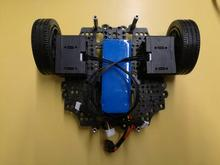
\includegraphics{Fig3.jpg}
        \caption{Level 1 assembly and arrangement}
        \label{fig:3}
    \end{figure}
\vspace{1em}
The level 2 waffle was placed directly on top of the motors and was supported by four rods and four screws. Once the waffle was secure, the OpenCR (32-bit ARM ® Cortex ® - m7) circuit board needed to be attached via four PCB support connectors. Wiring the OpenCR so that it can control both DYNAMIXEL motors as well as receive power presented a minor issue, the cables were in tight tension when both ends are in use. After manually adjusting and bending the cable to reduce tension on specific parts of it, we were able to properly establish a connection between the level 1 components and the OpenCR on level 2.\par
\begin{figure}[H]
        \centering
        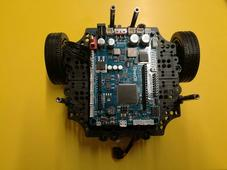
\includegraphics{Fig4.jpg}
        \caption{Level 2 assembly and arrangement}
        \label{fig:4}
    \end{figure}
\vspace{1em}
The third level was for the Raspberry Pi and USB2LDS boards, the Raspberry Pi will be used for wireless connectivity and data transference. The USB2LDS will connect to the LiDAR and allow it to transmit the raw data to make a Top down view of its surroundings. A similar issue was faced in terms of tension in the cables, the cables provided by ROBOTIS were short and needed to be manually bent in order to relieve a small fraction of the tension they are under. The USB2LDS cable is relatively thin and requires more attention when bending it, due to the established design of the TurtleBot3 there is not much that we can do about it, without a new design of the cable. We also implemented another camera on this level to allow manual control. In the scenario that you are on the master remote PC at the office and you need to send in a robot for manual surveillance and scouting of a building that is on fire, you will them have the ability to see what the robot does, visually inspect the surroundings and point out key interests.\par
\begin{figure}[H]
        \centering
        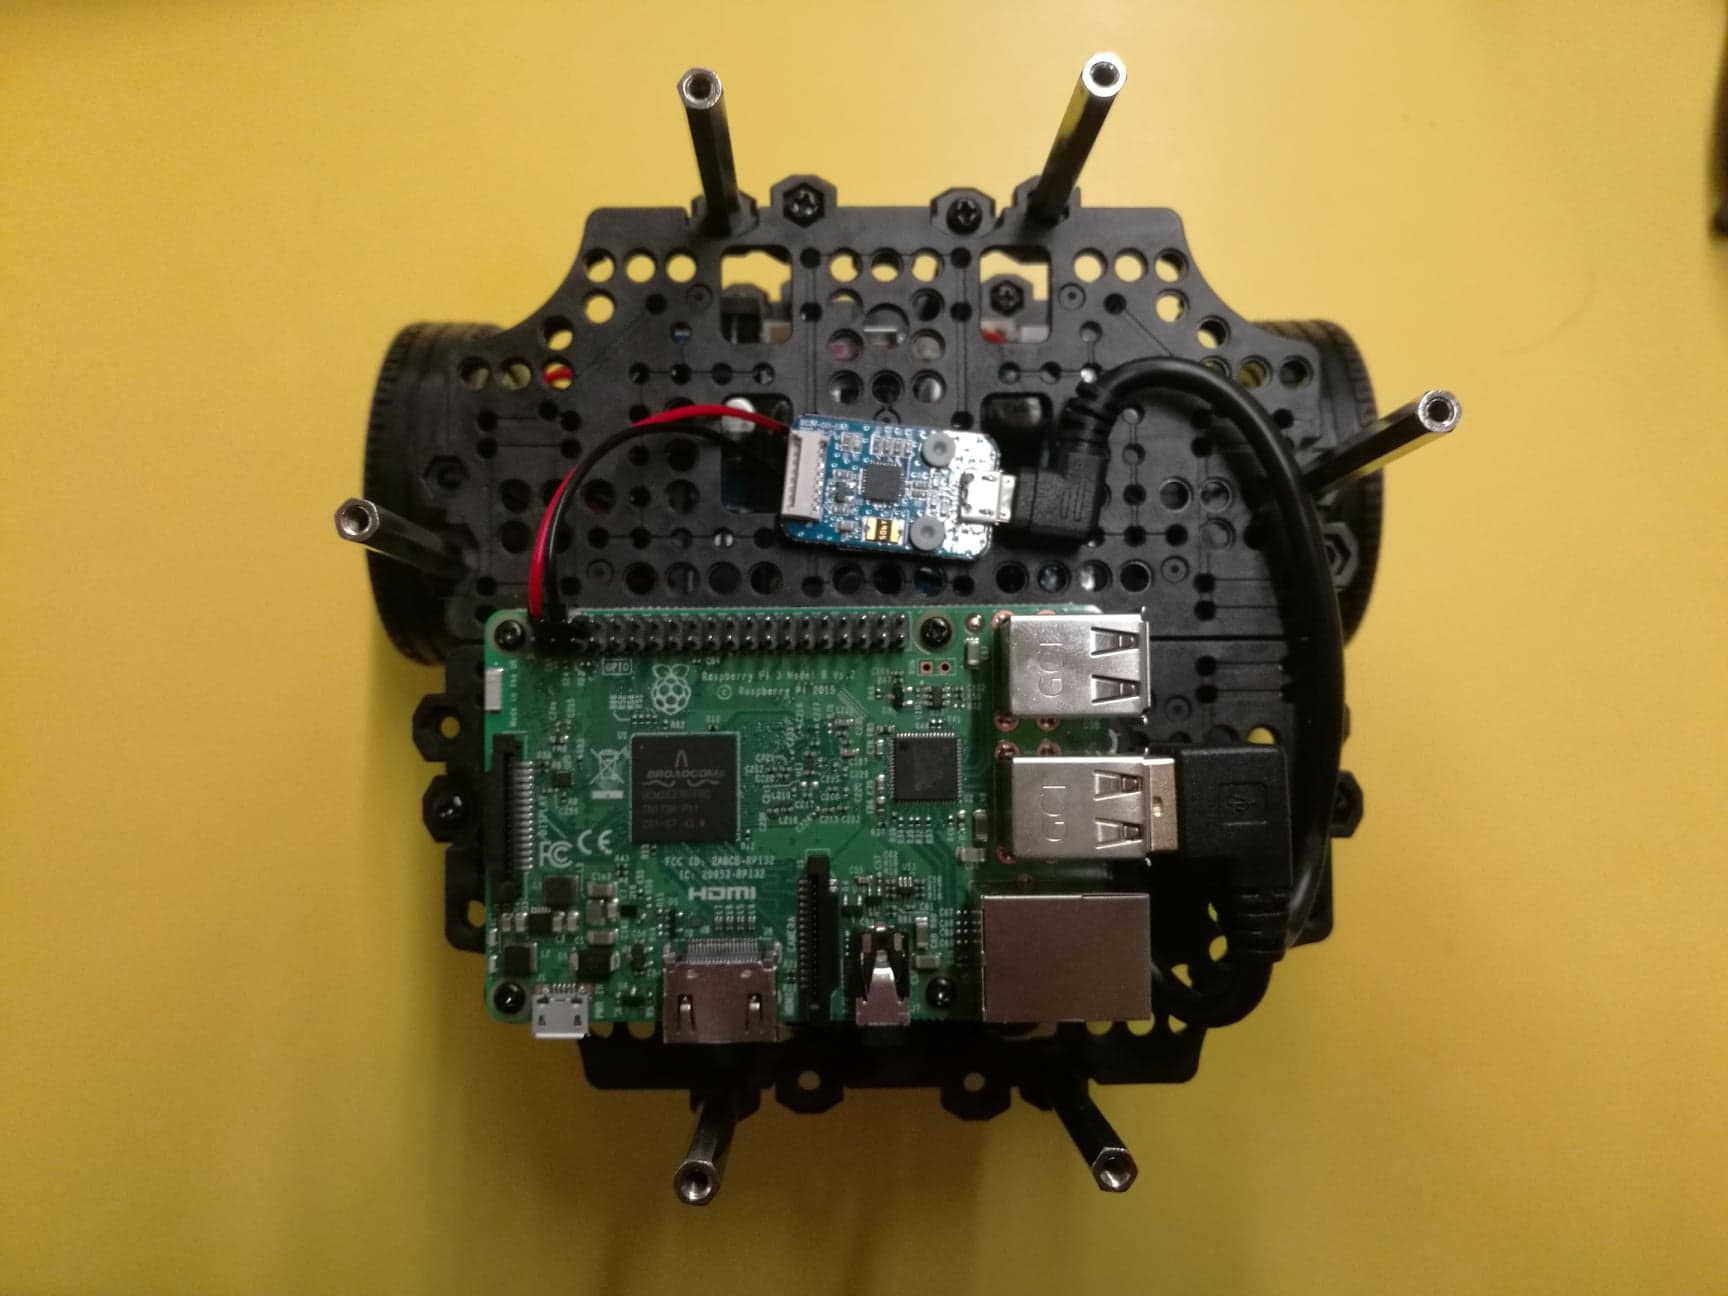
\includegraphics[width=0.45\textwidth]{Fig5.png}
        \caption{Level 3 assembly and arrangement}
        \label{fig:5}
    \end{figure}
\vspace{1em}
The fourth and final level (upper most level) of the Turtlebot3 has the 360\degree\  LiDAR for SLAM and Navigation. By having the LiDAR on the upper most level helps ensure that it will be able to see everything without any obstructions to its vision from its body. The LiDAR is connected via four PCB support connectors This method also brings forth an issue, being on the highest level means that it can not detect anything below itself as it establishes itself as the base level and records what it sees. To resolve this issue an additional camera was added to the third level, which will allow the TurtleBot3 to detect any obstacles that might be in front of it and below the LiDAR. The LiDAR was the final component of the assembly, the overall process was quite linear and did not consume a lot of time. Secondary testing was also done on the components as well, we wanted two testing phases to ensure that the components weren’t damaged after assembly as well.\par
\begin{figure}[H]
        \centering
        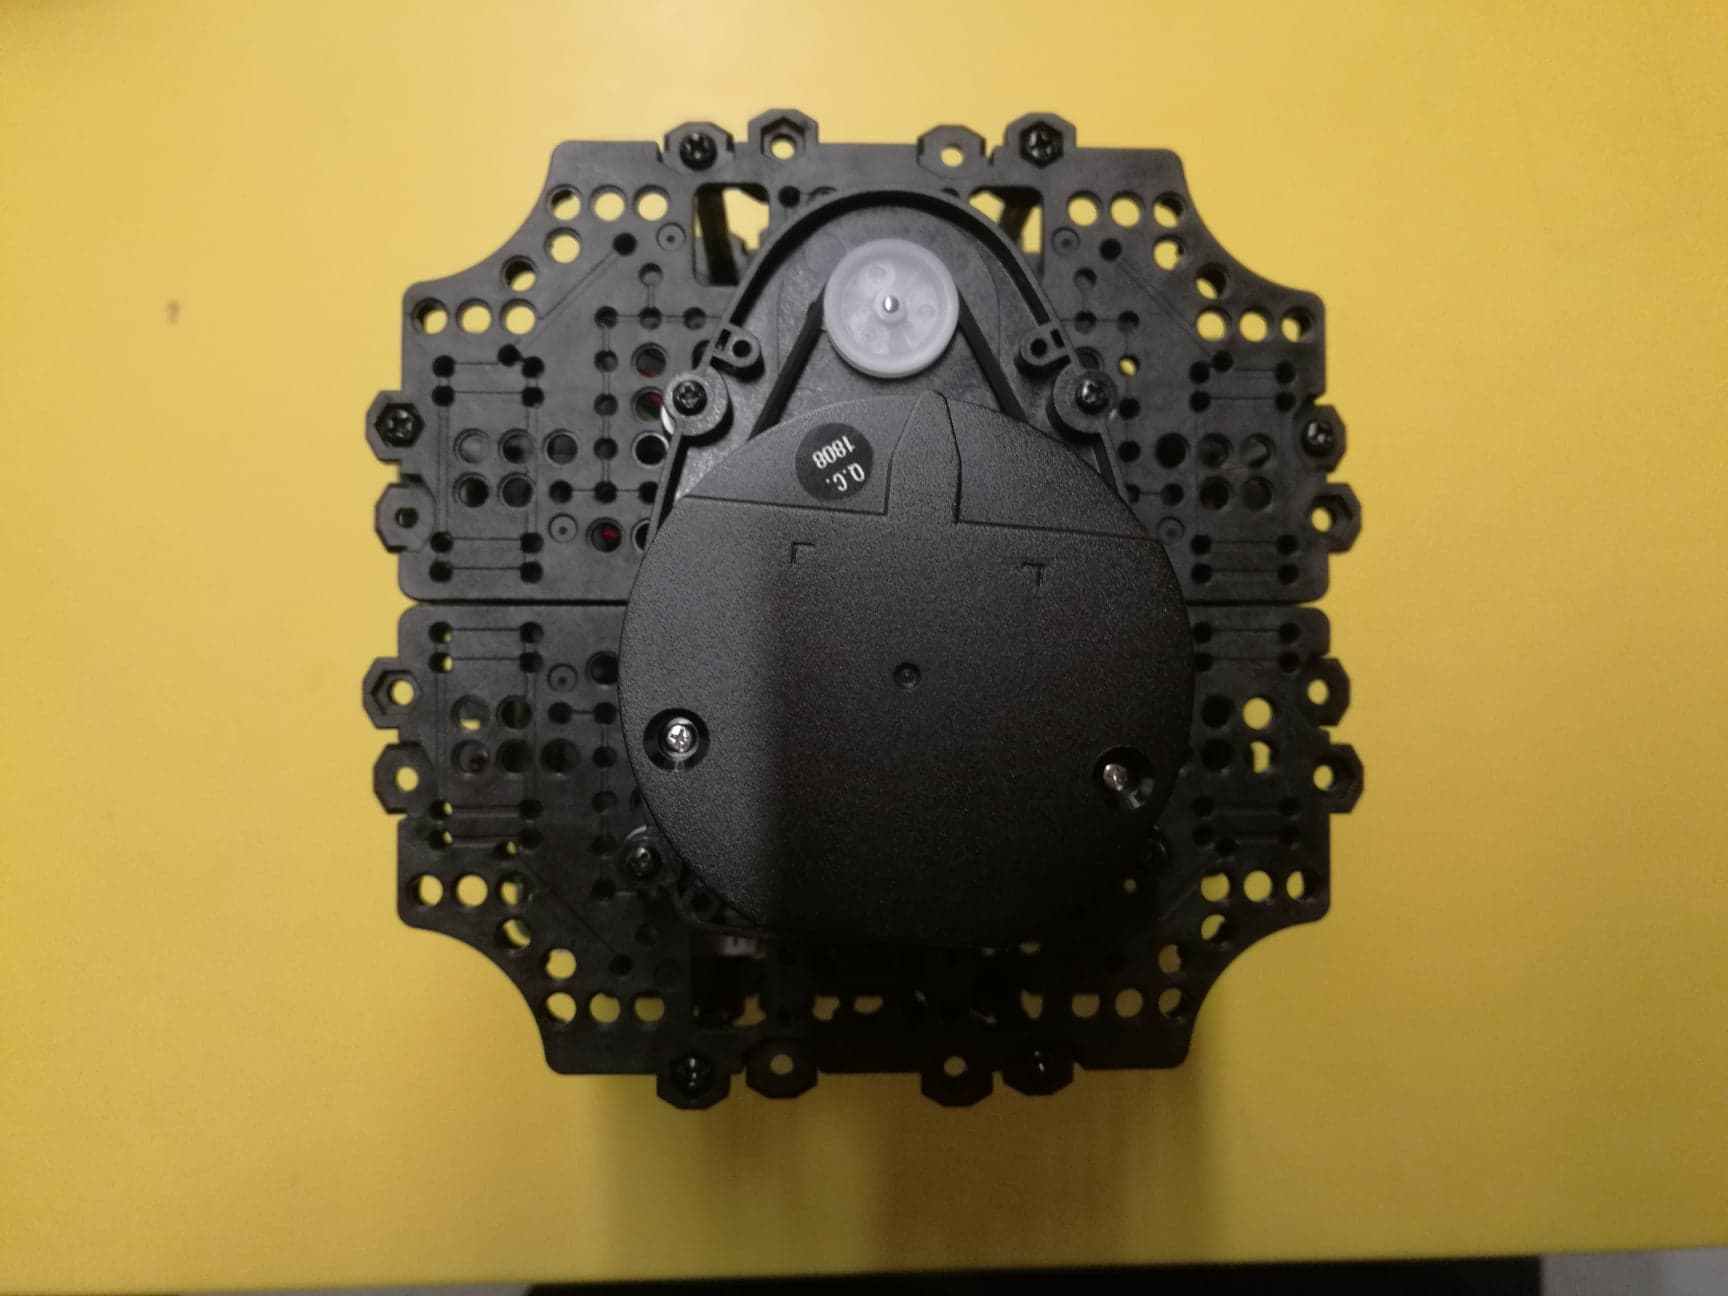
\includegraphics[width=0.45\textwidth]{Fig6.png}
        \caption{Level 4 assembly and arrangement}
        \label{fig:6}
    \end{figure}
\vspace{1em}
\vfill
\section{Robot Operating System (ROS)}
ROS is an open-sourced framework to write software for robotics. ROS includes tools, libraries and packages to program a robot and analyse its behaviour. In this project, ROS acts as intermediary between a user’s personal computer and the TurtleBot3’s Raspberry Pi as the latter’s computing unit. ROS can only be installed in Linux Operating System; hence the primary reason why the user’s PC should be a Linux machine. Since Raspberry Pi’s default operating system is based on Linux Ubuntu, ROS is an excellent framework to use for TurtleBot3.\par
\vspace{1em}
ROS provides numerous stacks necessary to program the robot. The stacks include files to run TurtleBot3’s sensors, servo motors, mapping algorithms, and simulations. Since ROS is community-maintained open-source framework, researchers and engineers may compile their own stacks to be used by other TurtleBot3 users. For example, one of the mapping algorithm being used in this project, Hector\_SLAM, is developed by a group of engineers from the Technical University of Darmstadt, Germany. ROS can be installed.\par
\vspace{1em}
In this project, the latest stable release of ROS, codenamed Kinetic Kame was used, installed onto a PC with a Linux Ubuntu MATE 18.2 operating system.\par

\section{Installation and Configuration on Linux Machine}

To install ROS on a typical Ubuntu machine, the command
\begin{minted}{bash}
$ sudo apt-get install ros-kinetic-desktop-full

\end{minted}
is to be issued to download and install the complete ROS stack. After ROS is installed, the command
\begin{minted}{bash}
$ source /opt/ros/kinetic/setup.bash

\end{minted}
should be issued in the terminal to run the script file unique to the Kinetic distribution of ROS. Next, the command
\begin{minted}{bash}
$ mkdir -p ~/catkin_ws/src

\end{minted}
is issued. The catkin\_ws directory will be where all ROS stacks, applications, and files will be located.\par
\vspace{1em}
As ROS is compatible with any robots that are programmable with Linux, it is important to configure the installed ROS to the files distributed by TurtleBot3’s manufacturer, Robotis. To do so, Robotis’ code repository from GitHub is to be cloned onto the catkin\_ws/src directory made earlier. The commands
\begin{minted}{bash}
$ git clone https://github.com/ROBOTIS-GIT/turtlebot3_msgs.git

\end{minted}
and
\begin{minted}{bash}
$ git clone https://github.com/ROBOTIS-GIT/turtlebot3.git

\end{minted}
are issued. To install the two repositories onto the ROS in the machine, the command
\begin{minted}{bash}
$ cd ~/catkin_ws && catkin_make

\end{minted}
is issued. The command catkin\_make compiles the code repositories and ensures their hierarchy and libraries are maintained in the machine as they are in the GitHub.\par
\vspace{1em}
The Linux machine will control the TurtleBot3 remotely through Wi-Fi. As such, the ROS should know the IP address of the machine. The setup shell file bashrc should be opened, and the following two lines should be added at the end of the file.
\begin{minted}{bash}
export ROS_MASTER_URI= http://192.168.10.100:11311
export ROS_HOSTNAME= 192.168.10.100

\end{minted}
The computer was assigned the IP address 192.168.10.100, hence the command. Whenever the IP address’s lease expires, or the TurtleBot3 is operated in a different network, the bashrc shell file should be modified to follow the correct IP address.\par

\section{Installation and Configuration on TurtleBot3}
Raspberry Pi 3 is the main computing unit of the TurtleBot3. For this project, the Raspberry Pi’s microSD card is preloaded with a burned image of Ubuntu Mate, using a normal PC and software such as Etcher. The Raspberry Pi should also be connected to the same Wi-Fi network with the Linux machine from the earlier section. With the Pi connected to the Internet, the same commands to install ROS should be issued from the Pi’s terminal window, with a few changes.\par
\vspace{1em}
After ROS is installed onto the Raspberry Pi, a driver file for the TurtleBot3 LIDAR should be downloaded by issuing the command
\begin{minted}{bash}
$ git clone https://github.com/ROBOTIS-GIT/hls_lfcd_lds_driver.git

\end{minted}
on the catkin\_ws directory. Another change is that the Pi does not need ROS packages such as SLAM, teleoperation, and simulation, as all of these packages would be run on the Linux Machine. To remove them, the commands
\begin{minted}{bash}
$ cd ~/catkin_ws/src/turtlebot3
$ sudo rm -r turtlebot3_description/ turtlebot3_teleop/ turtlebot3_navigation/ 
turtlebot3_slam/ turtlebot3_example/

\end{minted}
is issued.\par
\vspace{1em}

Similarly, the IP address of the Pi should also be added into its bashrc shell file. During the testing, the Pi was assigned the IP address 192.168.10.101. As such, the bashrc’s last two lines should be as follows.
\begin{minted}{bash}
export ROS_MASTER_URI=http://192.168.10.100:11311
export ROS_HOSTNAME=192.168.10.101

\end{minted}
It is important to note that only the ROS\_HOSTNAME reflects the IP address of the Pi, but not the ROS\_MASTER\_URI. This is because when ROS is activated at both the Linux computer and the Pi, the former will act as a Master computer, whereas the Pi will be the Slave. All commands to operate the TurtleBot3 will normally be issued from the Master computer.\par
\vspace{1em}

\section{Raspberry Pi Camera}
Camera is not included in the TurtleBot3 package. However, a camera would be useful as a modification to the robot. Since the robot is meant to be operated remotely, the user can navigate the robot safely. To do so, a Raspberry PI Camera v2 is installed as an external peripheral on the Raspberry Pi’s camera port.\par
\vspace{1em}
By default, Raspberry Pi does not allow a camera to take photography or stream videos, although the camera is already physically connected. To reconfigure the Pi, the command
\begin{minted}{bash}
$ sudo raspi-config

\end{minted}
is issued in the Pi’s terminal window. The camera’s can then be modified as an external input device for the Raspberry Pi. The Pi then must be restarted to complete the process. Upon rebooting, the Pi should then be able to take pictures. To test whether the camera functions, the command 
\begin{minted}{bash}
$ raspistill -v -o test.jpg

\end{minted} 
is issued, to take a photograph and save the picture in the PI’s home directory as “test.jpg”.\par
\vspace{1em}
Should there be no problems in testing the camera, the Raspberry Pi is ready to livestream a video into the remote Master’s browser. A Python script is needed, which is available in the appendix of this report. The Python script file is then be saved as rpi\_camera\_surveillance\_system.py. The script will feed the video to the Pi’s TCP port 8000. As such, to view the camera’s live video, the user controlling with the Master can open an Internet browser and type the address 192.168.10.101:8000. A sample of the camera’s live stream on the Master’s browser is shown in the Figure 4.5 below.
\begin{figure}[H]
        \centering
        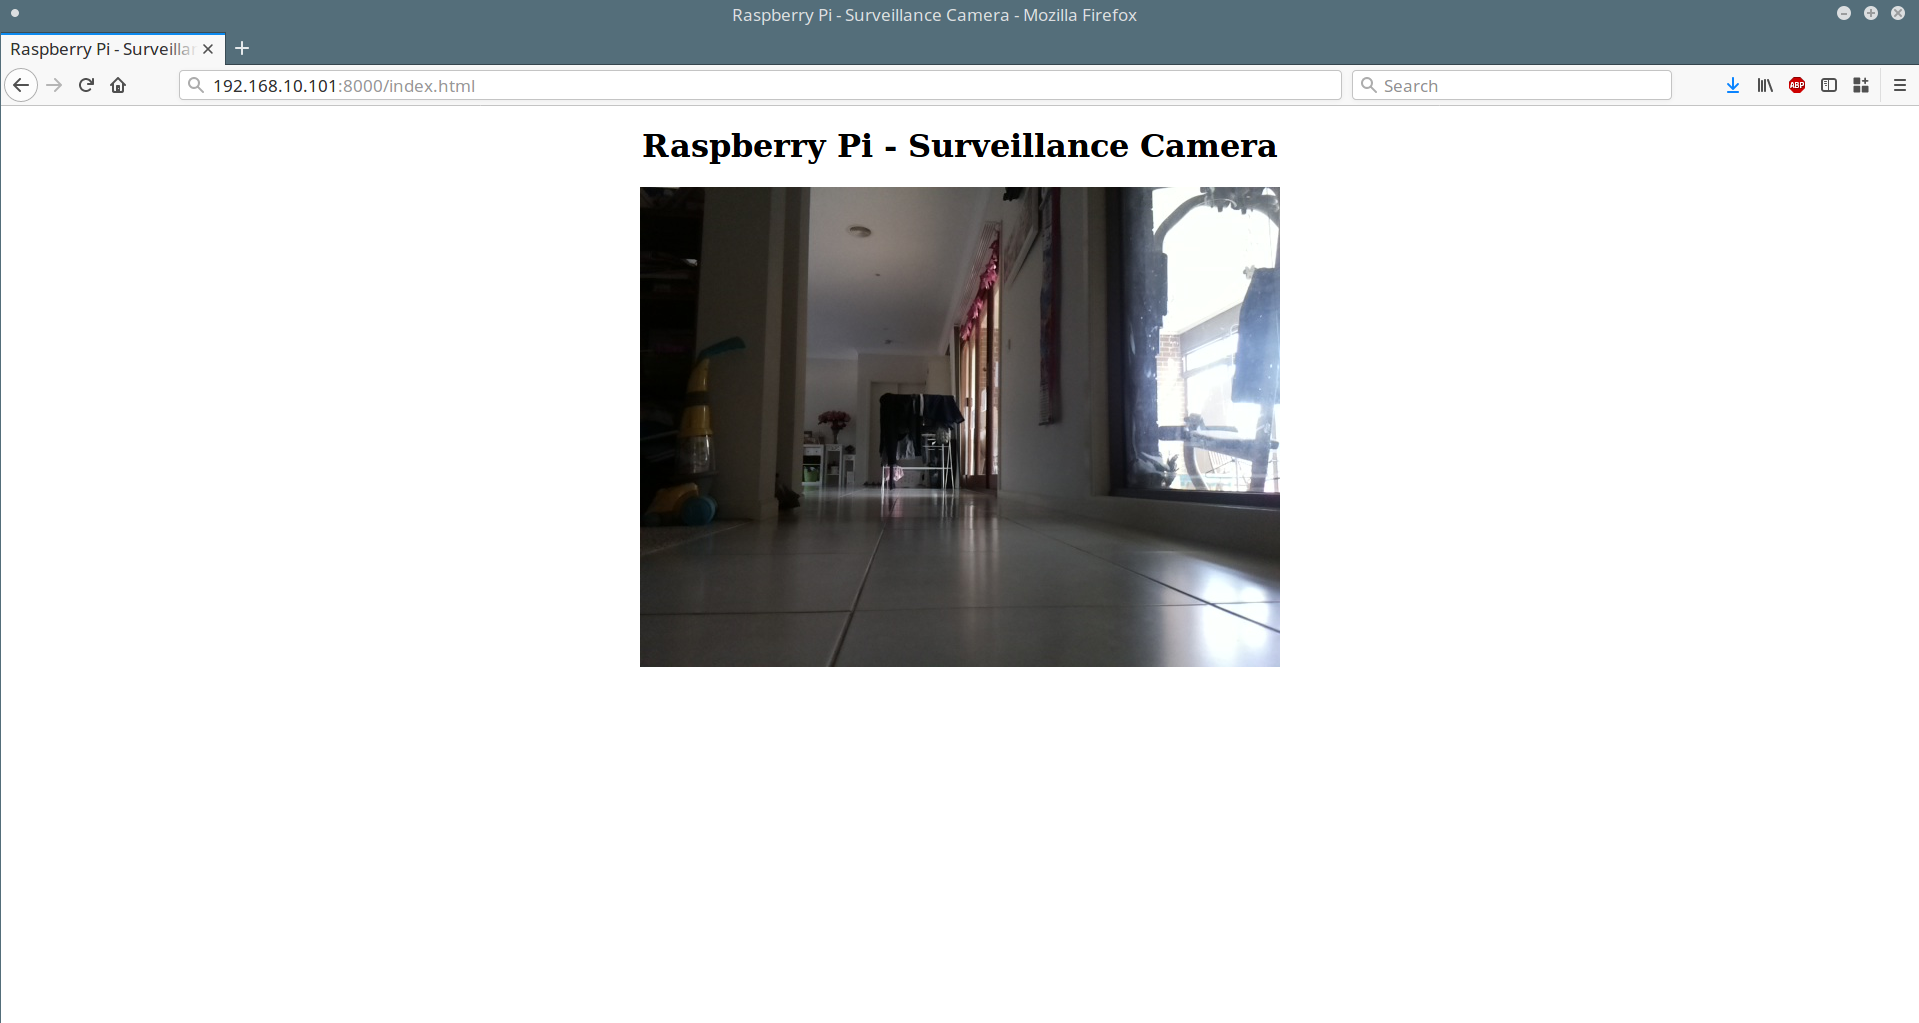
\includegraphics[width=0.95\textwidth]{Fig7.png}
        \caption{Live video stream from the Raspberry Pi Camera}
        \label{fig:7}
    \end{figure}
\section{RViz}
ROS Visualization is a 3D visualizer for displaying sensor data and state information from ROS.
RViz can also display live representations of sensor values coming over ROS Topics including Camera, depth cloud, effort, fluid pressure, grid, grid cells, illuminance, image, interactive makers, laser scan, map, maker, maker array, odometry, path, point cloud, pose, range, robot model, tf, temperature.\par
\vspace{1em}
All these qualities that RViz provide to the user makes it much easier to see and understand what the robot is seeing and thinking in the world around it hence making debugging much more easier to the user. The combination of ROS and RViz makes using simultaneous navigation and mapping (SLAM) easier to achieve.\par
\begin{figure}[H]
        \centering
        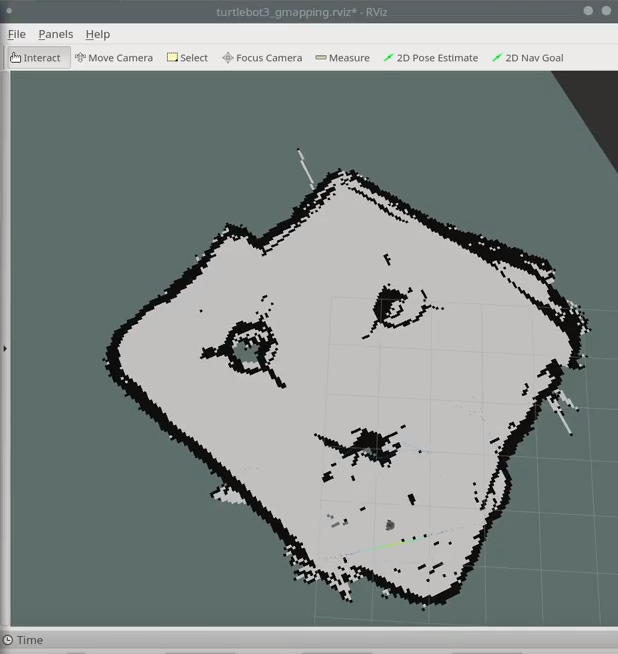
\includegraphics[width=0.45\textwidth]{Fig8.png}
        \caption{Rendering of map with RViz}
        \label{fig:8}
    \end{figure}
\vspace{1em}
The Figure 4.6 above shows the complete mapping of building 55 level 02 room 04 that is produced in RViz in this is why RViz is a very handy application to use since it provides the user with information of what the robot is seeing and what type of map is being produced while it moves around the room.\par
\vspace{1em}
\chapter{Discussion of Results and Findings}
The TurtleBot3 was tested mainly in RMIT’s Manufacturing Hub. The laboratory room was chosen due to its relatively small area but filled with chairs and desks, therefore suitable to examine the robot’s ability to avoid obstacles and the mapping algorithms’ accuracy.\par
\vspace{1em}
\section{Operating TurtleBot3}
In the Master computer’s terminal window, the command
\begin{minted}{bash}
$ roscore

\end{minted} 
is issued. This will activate the ROS package within the Master. At the same time, a Secure Shell (SSH) session is established to access the Slave’s terminal. In the Slave terminal, the ROS is similarly activated in the TurtleBot3, with the command
\begin{minted}{bash}
$ roslaunch turtlebot3_bringup turtlebot3_robot.launch

\end{minted} 
The two terminal windows will be left as it is during operating the TurtleBot3.\par
\vspace{1em}

To control TurtleBot3’s movement, a new terminal window is opened in the Master. The command to be launched is
\begin{minted}{bash}
$ roslaunch turtlebot3_teleop turtlebot3_teleop_key.launch

\end{minted}
This command allows the TurtleBot3 to be controlled using the Master’s keyboard. In the keyboard, pressing ‘W’ will drive the robot forward and increment its speed by approximately 10 cm/s. Pressing ‘X' reverses the direction by 10 cm/s. Pressing ‘A’ or ‘D’ will turn the robot’s heading towards the left or right respectively by 0.01 rad/s.\par
\vspace{1em}

\section{Drawing Maps}
While keeping all previous terminals open, another terminal should be opened to launch the SLAM algorithm. The command to be issued in the new Master’s terminal is \begin{minted}{bash}
$ roslaunch turtlebot3_slam turtlebot3_slam.launch.

\end{minted}
The terminal will display a stream of the robot’s pose, and starts an RViz instance showing the robot and the obstacles around it. To build the map to a larger area, the teleop\_key.launch terminal used to control the robot’s movement is reopened. RViz will update the map accordingly.\par
\vspace{1em}
By default, the turtlebot3\_slam will build a map with gmapping algorithm. To draw a map with other algorithms, for example with Hector\_SLAM, the command to be issued should be 
\begin{minted}{bash}
$ roslaunch turtlebot3_slam turtlebot3_slam.launch slam_methods:=hector

\end{minted}

\section{Comparison of SLAM Methods}
Gmapping algorithm assumes that the robot’s initial pose in an imaginary Cartesian plane to be located on the origin, that is (0, 0, 0). The first 2 coordinates are the (x,y) coordinates, with the angle where the robot is heading is represented as the third number. The gmapping algorithm then will determine the robot’s nearby obstacles such as wall and furnitures, and draw them accordingly based on the information provided by the scanning of the Lidar. As such, the gmapping’s iteration of the robot’s pose can be illustrated in the table below.\par

\begin{table}[H]
    \centering
    \begin{tabular}{cccccc}
         X$_{1}$ & X$_{2}$ & X$_{3}$ & ... & ... X$_{n}$ \\
         Y$_{1}$ & Y$_{2}$ & Y$_{3}$ & ... & ... Y$_{n}$ \\
         $\theta_{1}$ & $\theta_{2}$ & $\theta_{3}$ & ... & ... $\theta_{n}$ \\
         
    \end{tabular}
    \caption{Poses information streamed by gmapping}
    \label{tab:my_label}
\end{table}
The second method tested in this project, Hector\_SLAM, does not take into account the Lidar’s scanning to determine the robot’s pose. Instead, Hector\_SLAM reads into the robot’s odometry. To do so, the algorithm reads into the Dynamixel’s encoding to determine the robot’s position. In the scope of this project, the robot is mainly tested within RMIT University’s Mechatronics Lab, Building 55 Level 2 Room 4. The actual map of the room during the testing was sketched with a computer aided design software, as shown by the Figure 5.1 below.\par
\begin{figure}[H]
        \centering
        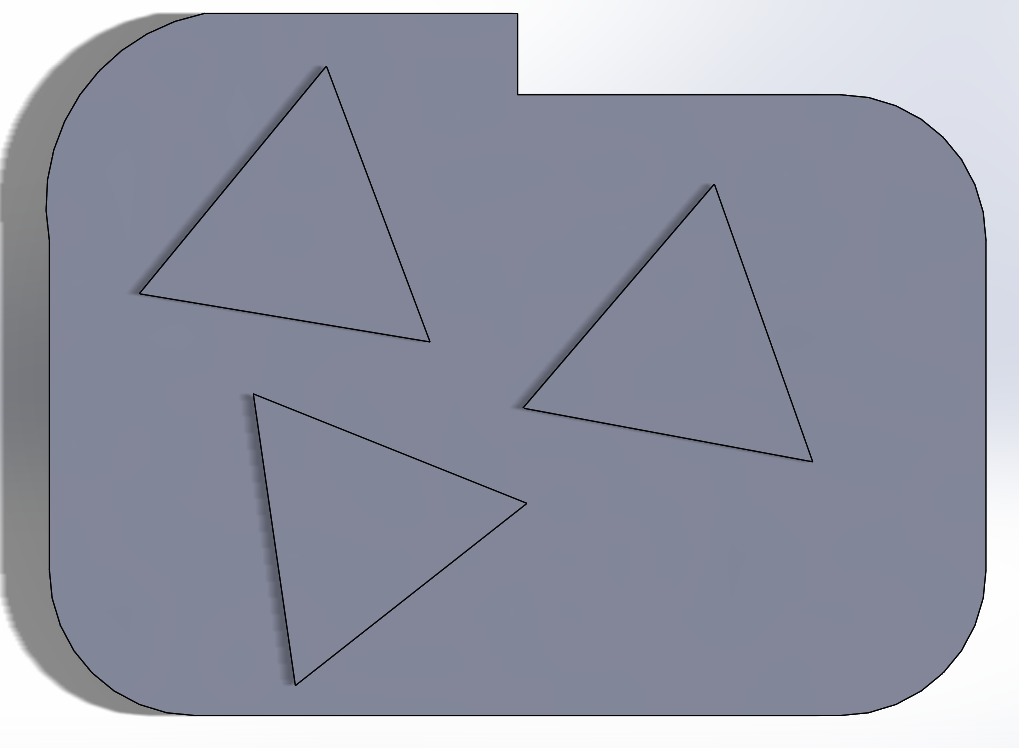
\includegraphics[width=0.75\textwidth]{Fig9.png}
        \caption{Sketched map of the testing laboratory for comparison}
        \label{fig:9}
    \end{figure}

The room consists of 3 triangular desks supported by circular bases. Since TurtleBot3’s Lidar only captures obstacles at the same height where the Lidar is positioned on the robot, only the desks’ bases were captured in RViz. The map rendered with gmapping algorithm is shown in the Figure 5.2 below.\par
\begin{figure}[H]
        \centering
        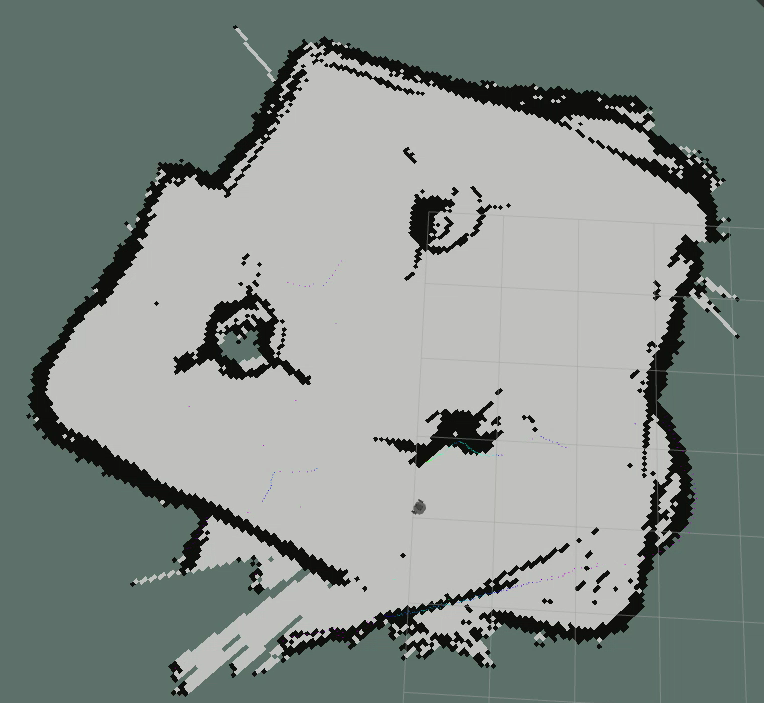
\includegraphics[width=0.65\textwidth]{Fig10.png}
        \caption{Map rendering with Gmapping algorithm}
        \label{fig:10}
\end{figure}
\vspace{1em}
In comparison, the map rendered by Hector\_SLAM algorithm can be seen in the Figure 5.3 below.\par
\begin{figure}[H]
        \centering
        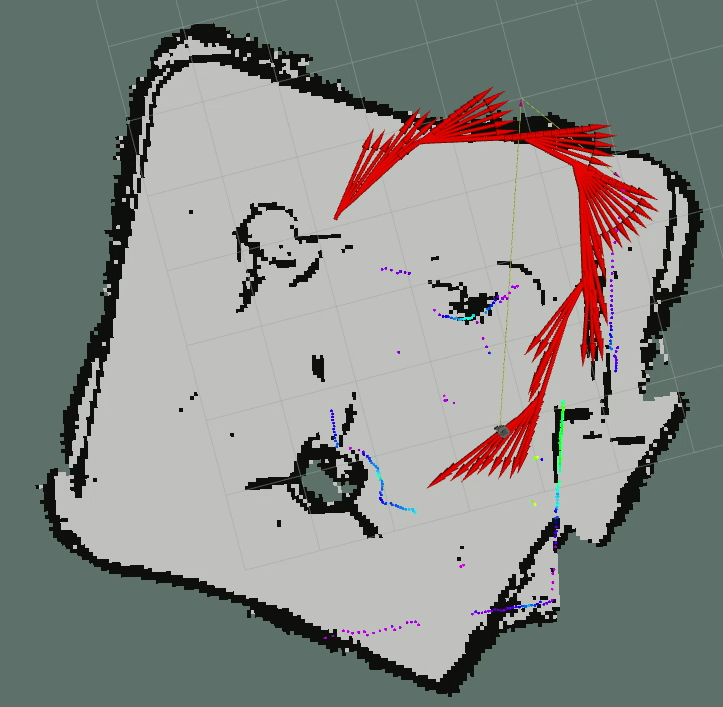
\includegraphics[width=0.65\textwidth]{Fig11.png}
        \caption{Map rendering with Hector\_SLAM algorithm}
        \label{fig:11}
\end{figure}
In both maps, the black lines are the obstacles as seen by the Lidar. The light gray shows empty spaces where there are no identified obstacles. The area of the room was approximately 50 square meter, and gmapping algorithm requires 13 minutes to draw the map, whereas Hector\_SLAM needed 10 minutes and 15 seconds to do so. During both processes, a screen recorder is activated to better show how the map was built by the two algorithms. The video has been uploaded onto YouTube, which links have been included in the Appendix 2 of this report.\par
\vspace{1em}
From the gathered data, it is inconclusive to determine which algorithm is objectively better in all settings and scenarios. Gmapping algorithm can be disorienting for the robot when the surrounding obstacles are not inanimate, for example walking passersby or moving obstacles. Since Hector\_SLAM relies on encoded data from the Dynamixel servo motor, the algorithm is not suitable when the robot is operated on rough, uneven surfaces such as carpeted ground. The robot’s slippage causes Hector\_SLAM to draw the map inaccurately.\par
\vspace{1em}

\section{Comparison of Similar Robots}
In this particular industry there are other competitors with similar or different variations to the modular solutions that what we offer, they promote robots that operate by moving through the air rather than ground movement.\par
\begin{figure}[H]
        \centering
        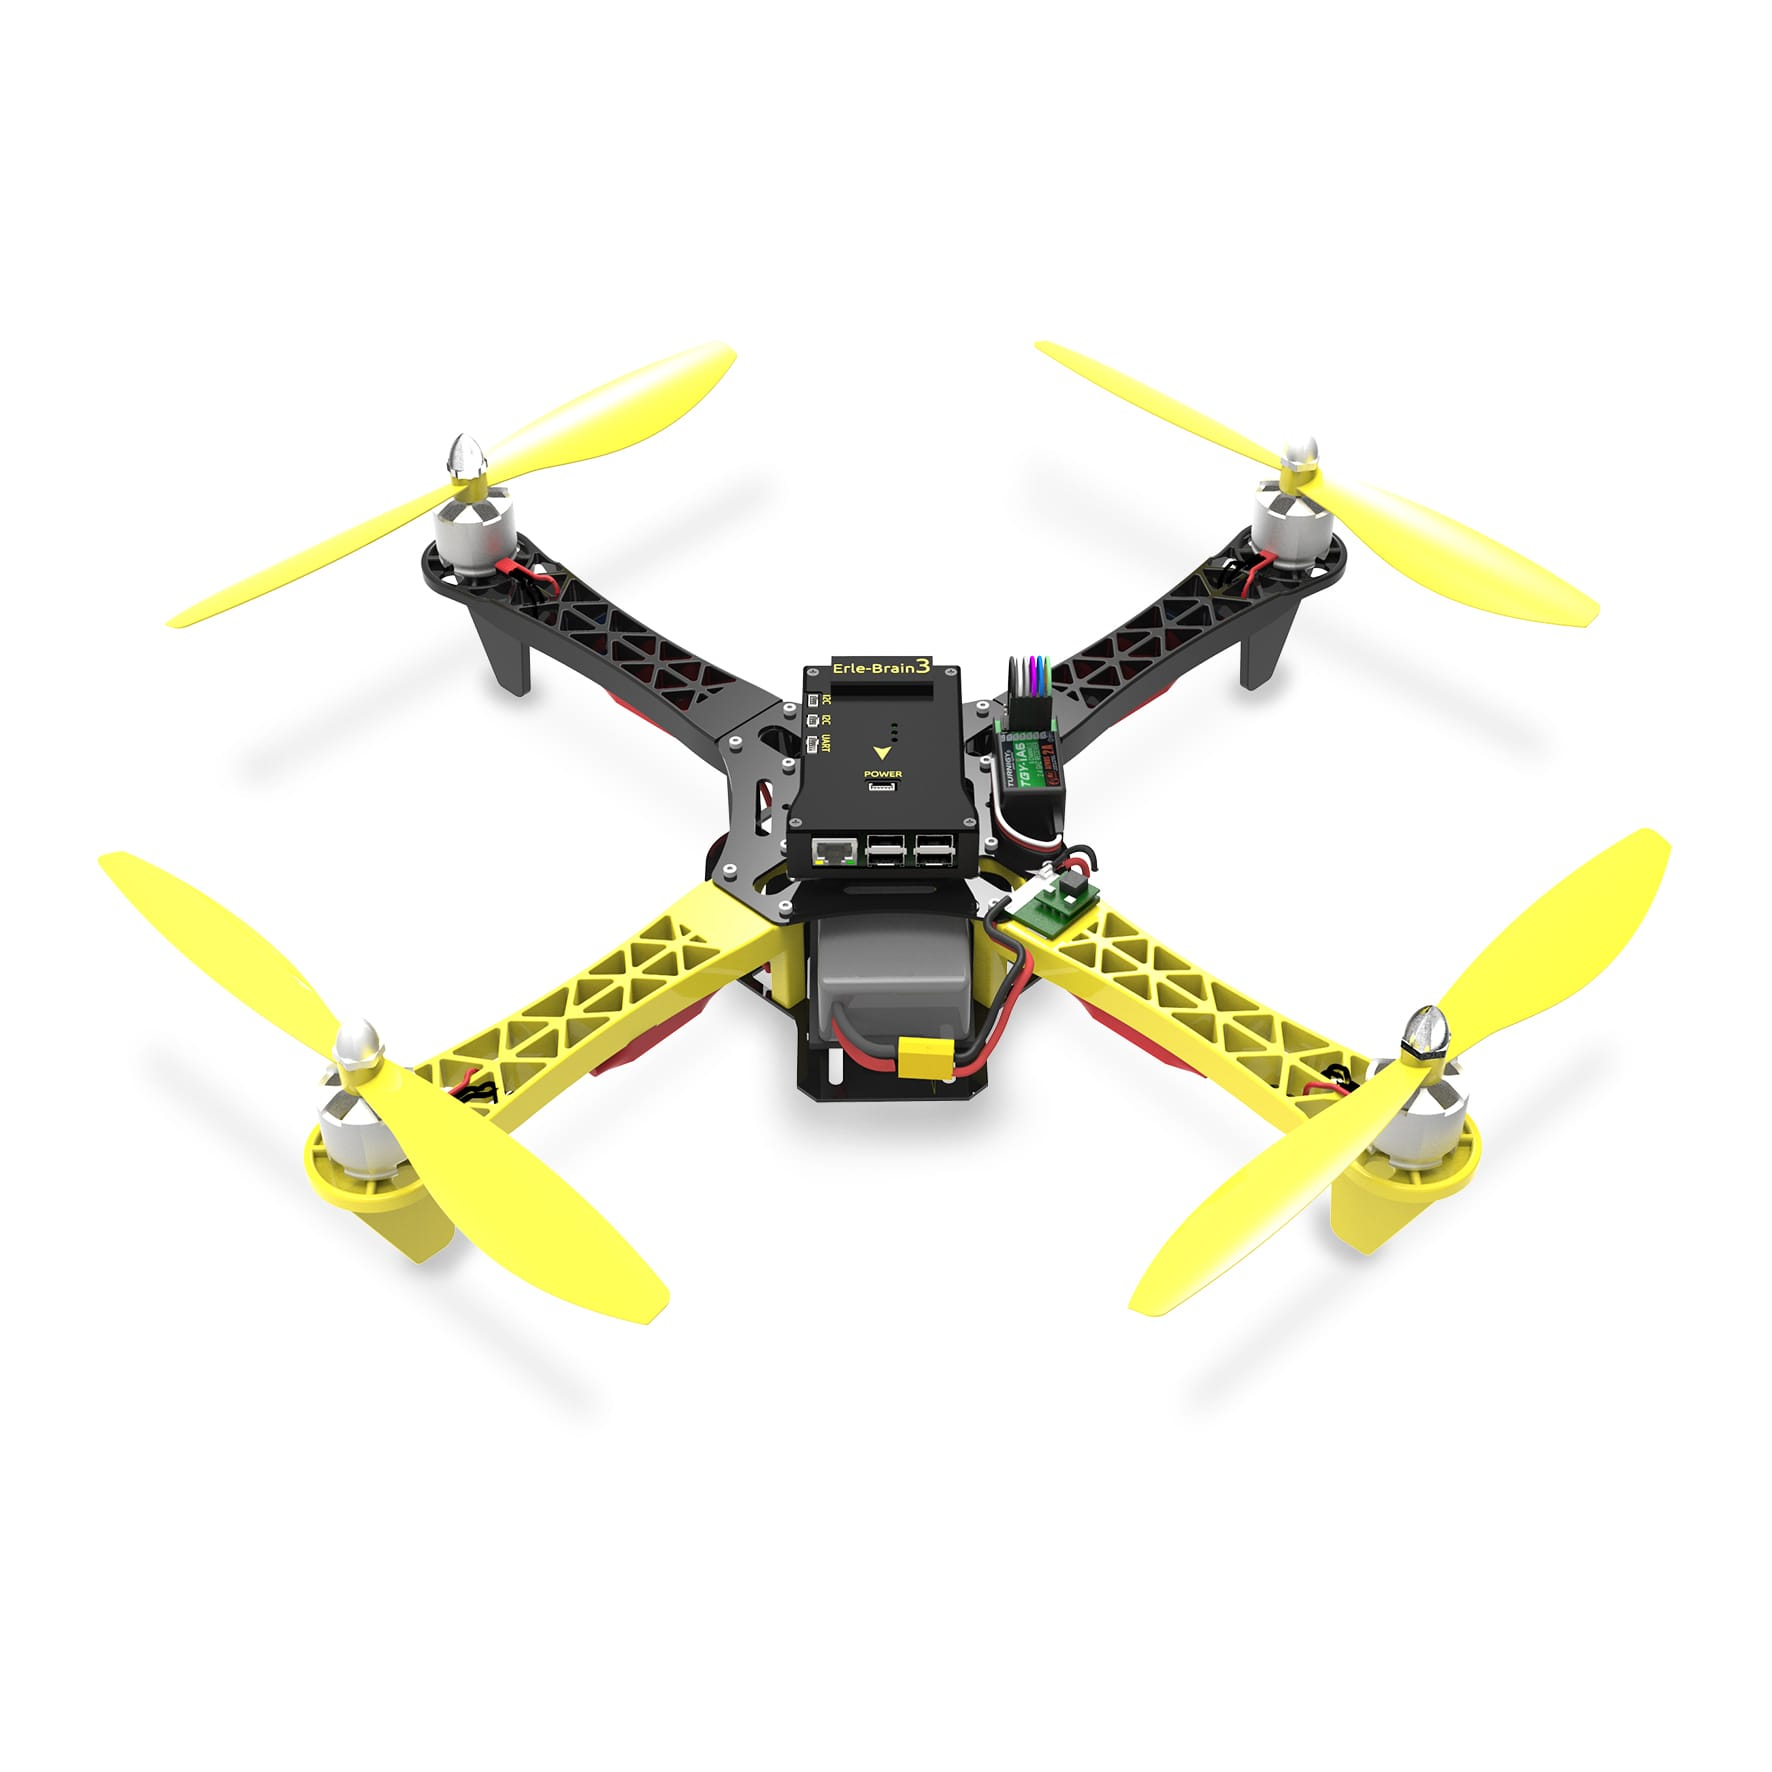
\includegraphics[width=0.55\textwidth]{Fig12.png}
        \caption{ERLE-COPTER drone kit from Erle Robotics}
        \label{fig:12}
\end{figure}
This particular method is quite conventional as there are certain advantages to this modular solution. Aerial robots can access locations and navigate them quite easily. Due to their flying capabilities which allows them to fly lower and in more directions, therefore resulting in more freedom and less movement restrictions in comparison to ground robots. They can be deployed from any location and being mapping immediately. Being airborne means that any obstacles stemming upwards from the ground up will be mapped and visualised in a 3 dimensional map where the Z-coordinate is used.\par
\begin{figure}[H]
        \centering
        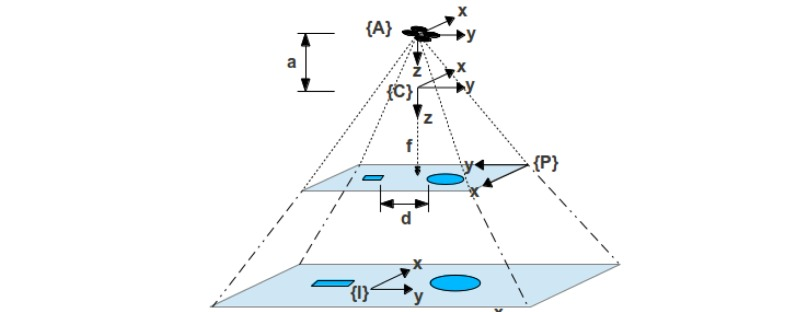
\includegraphics[width=0.8\textwidth]{Fig13.png}
        \caption{Coordinate frames from “An Aerial–Ground Robotic System for Navigation and Obstacle Mapping in Large Outdoor Areas“}
        \label{fig:13}
\end{figure}
\vspace{1em}
Figure 5.5 above demonstrates an aerial robot mapping the surrounding area below it and taking into account the obstacles marked in blue. The first layer, the image plane (I) has the distance between the two obstacles (d) and the X,Y,  position from them. The second layer, labelled the Pixel plane receives the data, reduces the size of the first layer and has the X,Y,Z position from the camera frame (C), which then ties in directly with the Aerial frame (A) and maps the position in relation to the previous levels data. As advantageous as this is there are external factors which affect the performance of the drone and its mapping and navigational capabilities. Variables taken into account can range from changes in weather, wind direction/speed, battery power, hardware sizes and strains, possible malfunctions, precipitation, humidity, snow etc. Variables that don’t affect ground robots include changes in weather as the ground robots can be configured for all types of weather, wind conditions as well do not have that much of an effect as well. Variables such as battery power, hardware sizes and strains possible malfunctions are variable that do affect the ground robot as well but not to a a large extent as it does with aerial robots. Precipitation wouldn’t be able to affect a robot operating on the ground as the robot will be using caterpillar treads to move through the terrain.\par
\begin{figure}[H]
        \centering
        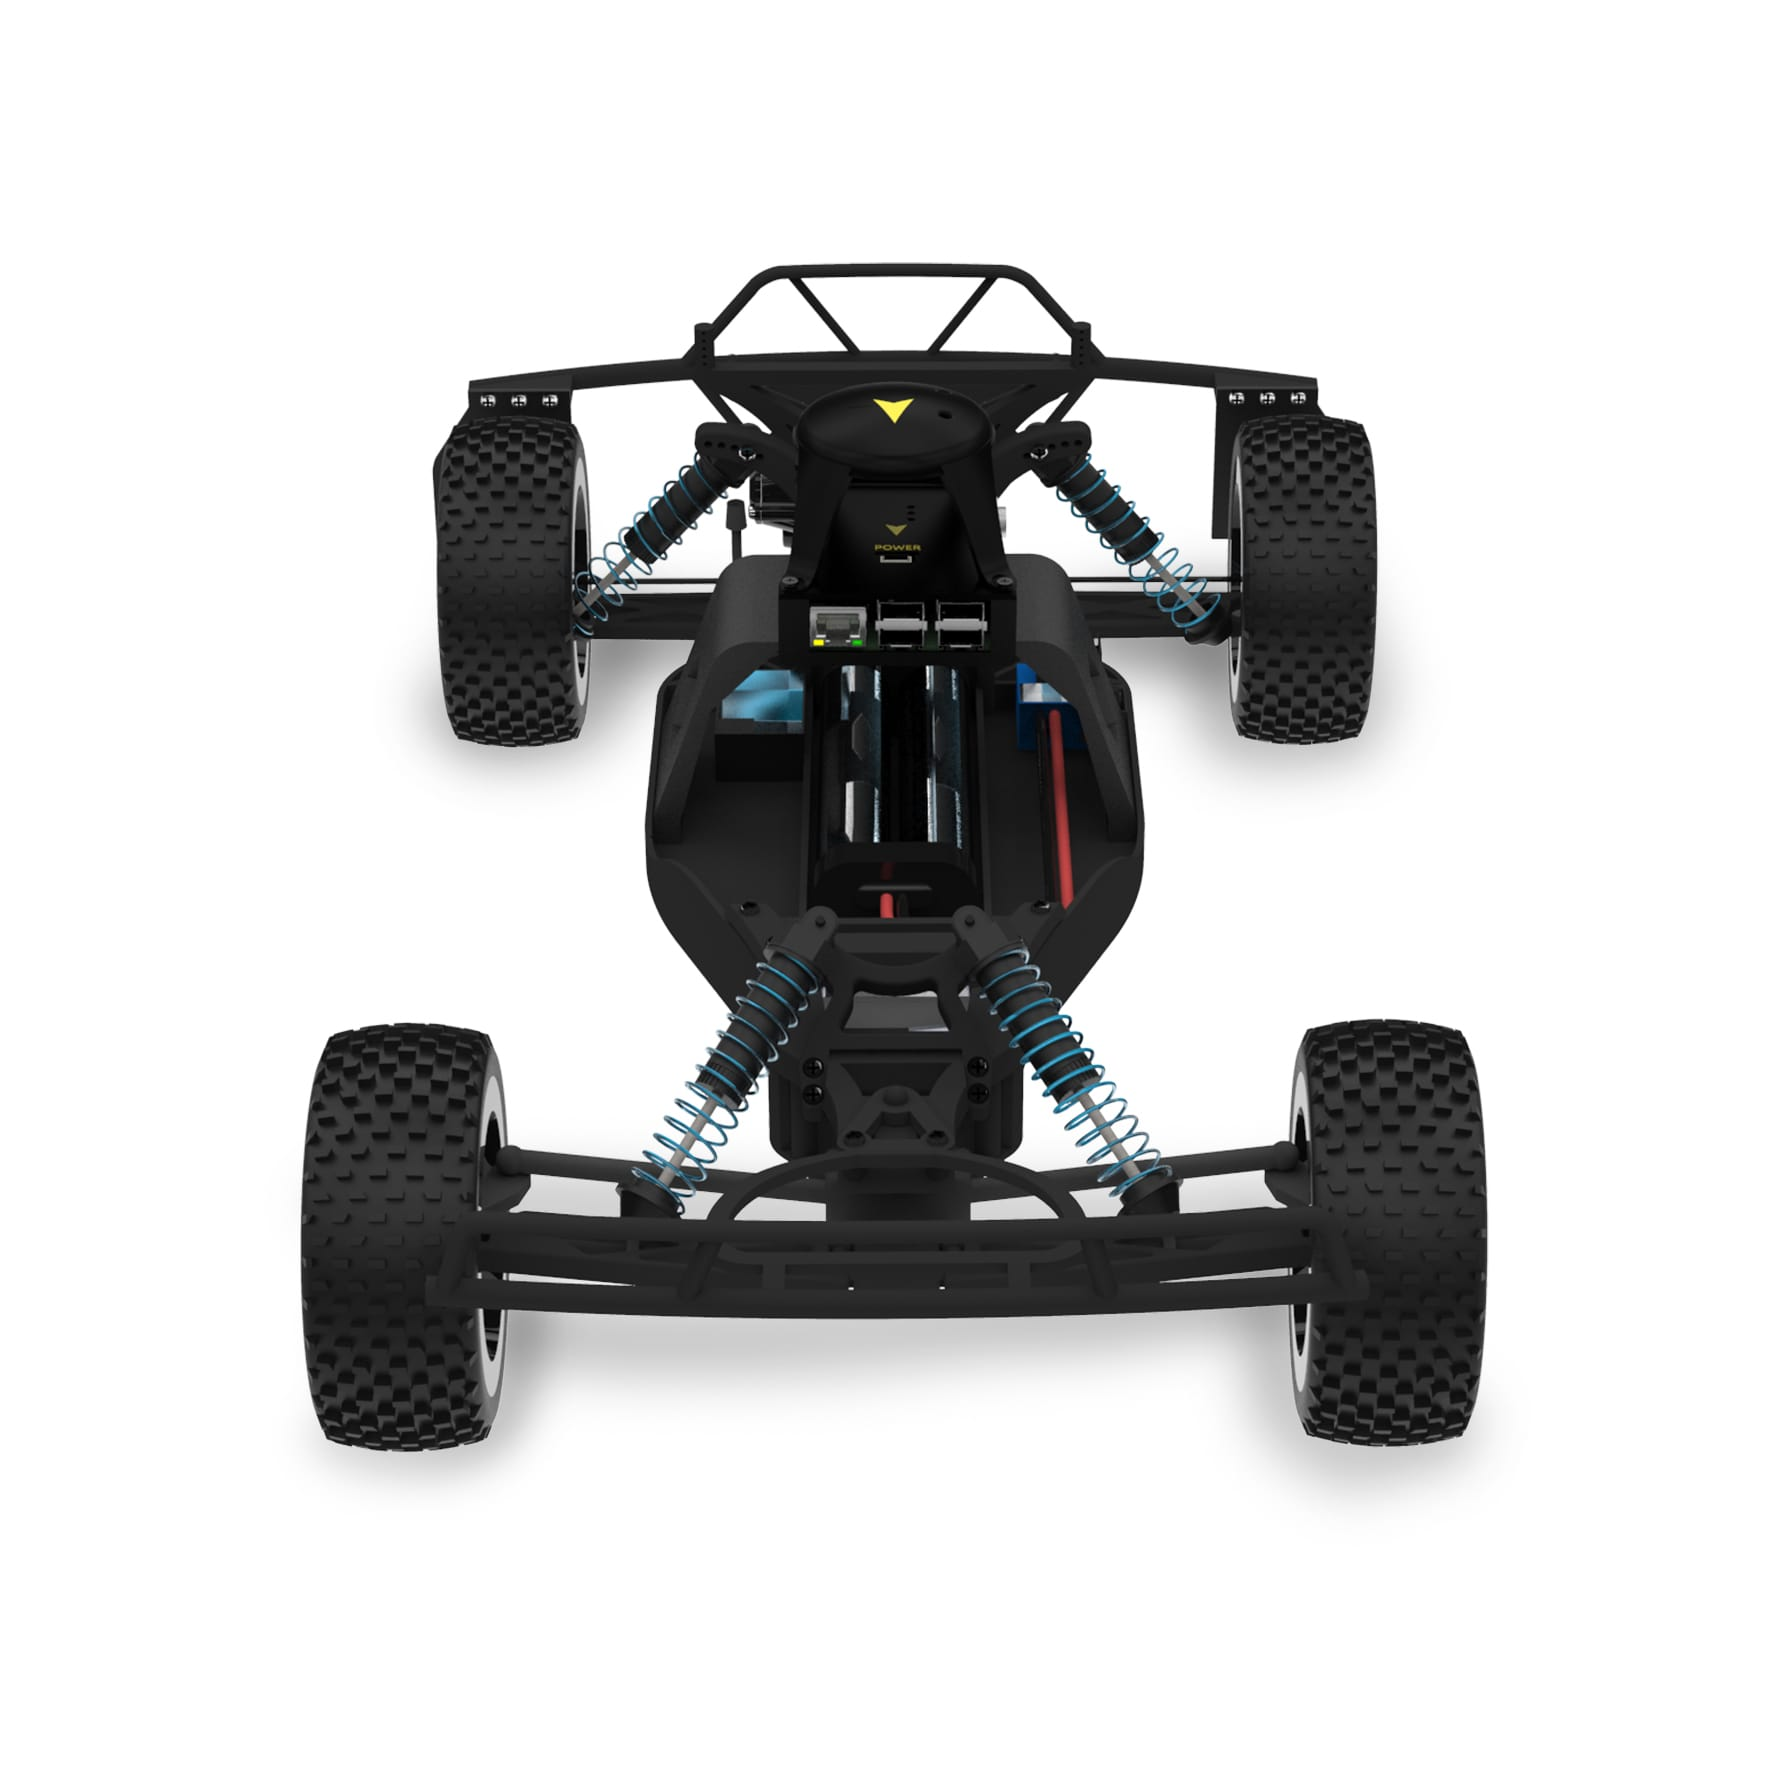
\includegraphics[width=0.45\textwidth]{Fig14.png}
        \caption{ERLE-ROVER from Erle Robotics}
        \label{fig:14}
\end{figure}
\vspace{1em}
When comparing other robots on the market with our modular ones, various factors need to be taken into account, size would be one of them. A larger grounded robot will need a larger battery, larger motors and frame. A larger frame doesn’t equate to a better robot, the mobility of the solution would be at risk. A larger robot would have trouble autonomously navigating a rough terrain area in comparison to a smaller more optimized version of the robot would be more than capable of doing the task. Our goal is to solely focus on movement on the ground to an acceptable premise as there is not a lot of external factors to focus on.\par
\vspace{1em}
In relation to size, the design must also be criticized. A small robot may be optimal but if the design is poor then the robot will suffer as a result. As seen in Figure 5.7 below the ERLE ROVER has been designed for outdoor mapping and navigation, this particular design is not optimised for traversing rough terrain due to the frame and tires. The frame is quite light which can result to the robot flipping if encountering an awkward angle on the terrain floor and choosing to still move forward.\par
\begin{figure}[H]
        \centering
        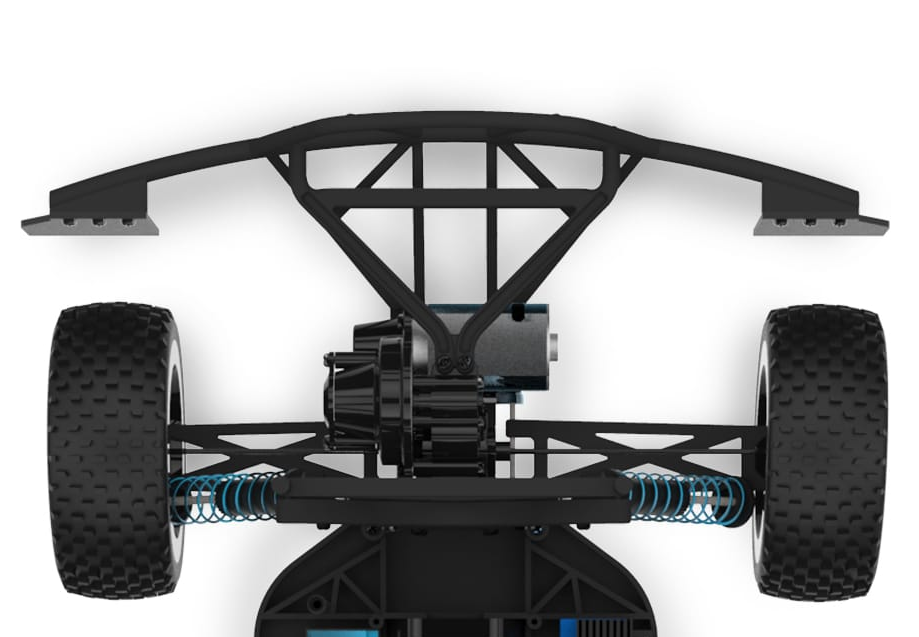
\includegraphics[width=0.45\textwidth]{Fig15.png}
        \caption{Zoomed in image of the single motor}
        \label{fig:15}
\end{figure}
\vspace{1em}
Using one motor for two wheels results in low torque, a more optimised solution to this problem would be for two motors, one motor would control two wheels using a caterpillar tread. The type of wheel is another issue to be addressed, having four individual wheels grouped into two means that each set would have to overcome a tough incline. The size of the body can become stuck/damaged if the robot encounters and sudden change in ground level as the rear wheels would still push the robot forward while the body is grazing the ground floor. If any of the wheels fail then the mobility will experience a big loss, changing the rounder wheels for caterpillar treads removes this issue, as illustrated by Figure 5.8 below.\par
\begin{figure}[H]
        \centering
        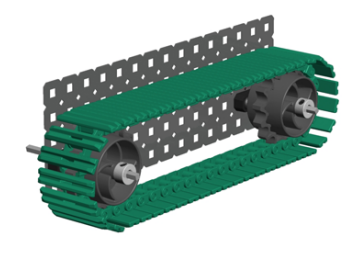
\includegraphics[width=0.45\textwidth]{Fig16.png}
        \caption{Basic track profile}
        \label{fig:16}
\end{figure}
\vspace{1em}
Caterpillar treads ensure that the robot will be able to cope with sudden changes in ground level without damaging the main body, as well as being able to traverse over obstacles to map the surrounding areas in comparison to round wheels.\par

\chapter{Risk Assessments}
The risks identified in the project are listed as the following.\par

\begin{enumerate}
    \item \textbf{Traffic Hazard} \\
    TurtleBot3’s movements can be controlled remotely, hence unaware passersby may trip on the moving robot. Users operating the robot unaware of the environment/surroundings of the robot may operate the robot to outdoor surfaces (i.e. soil/body of water). To alleviate the risk, the robot shall be Operated only within a restricted space and its movement will be monitored in person. This risk is also the reason why Raspberry Pi Camera is installed to the front side of the robot. Finally, nearby passersby will be alerted when the robot is operated.\par
    \item \textbf{Electrical Hazard} \\
    The robot may not be connected to the power outlet properly during charging. This risk can be reduced by only charging the TurtleBot3’s battery in the prepared power mains in the laboratory or during the exhibition.\par
    \item \textbf{Fire Hazard} \\
    	Due to the utilisation of an 11.1V Lithium-Polymer (Li-Po) battery as the TurtleBot3’s power supply, proper handling process must be observed carefully. Li-Po batteries can explode and burn all of the cells when charged incorrectly. Since the battery is essential and cannot be substituted, the risk can only be reduced by alleviating the impact should any accident happen. To do so, a Li-Po handling bag will be used to transport the battery, as well as preparing a bucket of sand as the battery’s disposal in the event of explosion. The operators of the robot should also be aware of where the dry chemical fire extinguishers are located when operating the TurtleBot3.\par
\end{enumerate}

\chapter{Timeline Project Plan}
\begin{table}[H]
\centering
\begin{tabular}{|l|l|r|r|}
\toprule
              & \textbf{Task}                     & \textbf{Start Date}   & \textbf{Finish Date} \\
\midrule
1 & Installing Linux Ubuntu Mate on Raspberry Pi                  & 30/07/2018    & 30/07/2018                           \\ \hline
2 & Assembly on TurtleBot3       
            & 31/07/2018    & 31/07/2018            
              \\ \hline
3 & Drafting Project Plan
            & 30/07/2018    & 1/08/2018                 \\ \hline
4 & Finalizing Gantt Chart
            & 1/08/2018     & 6/08/2018                 \\ \hline
5 & Submission of Gantt Chart (Assignment 1)                      & 6/08/2018     & 6/08/2018                             \\ \hline
6 & Programming OpenCR Board
            & 1/08/2018     & 13/08/2018
              \\ \hline
7 & First test of main system
            & 13/08/2018    & 27/08/2018
              \\ \hline
8 & Mounting Raspberry Pi Camera 
            & 27/08/2018    & 27/08/2018
              \\ \hline
9 & Comparing and Implementing SLAM algorithms
            & 16/08/2018    & 30/08/2018                \\ \hline
10 & Drafting final report
            & 23/08/2018    & 8/10/2018
              \\ \hline
11 & Preparing EnGenius exhibition supporting materials   & 24/09/2018    & 16/10/2018                            \\ \hline
12 & Final tests and preparation for EnGenius                     & 9/10/2018     & 16/10/2018                            \\ \hline
13 & EnGenius Exhibition and Presentation 
            & 17/10/2018    & 17/10/2018
              \\ \hline
\bottomrule
\end{tabular}
\label{tab:Table 7.1}
\caption{Project scheduling}
\end{table}
\begin{figure}[H]
        \centering
        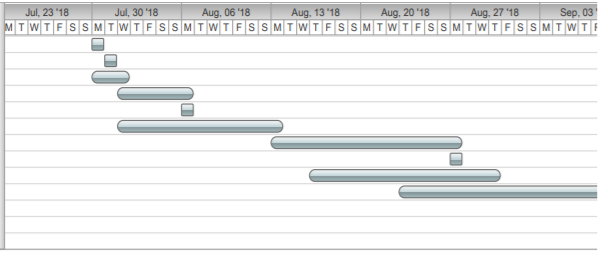
\includegraphics[width=0.95\textwidth]{Fig17.png}
        \caption{Gantt chart for project schedule}
        \label{fig:17}
\end{figure}
\vspace{1em}
\chapter{Conclusion}
In conclusion learning the way to operate ROS and find different algorithms to get the most accurate map possible mapped out with Rviz we came to a conclusion that Hector\_SLAM is the preferred method and algorithm because the maps in comparison to Gmapping was more accurate and we have two links to the videos of both Hector\_SLAM and Gmapping that shows the creation of the map live. We have also concluded that the Robot can move autonomously but it needs a sense of direction meaning it need to be given the first coordinate for it to move too and from there it can move around autonomously and map the environment around it.\par

\chapter{Future Works}
It is possible to create more accurate maps of an indoor setting with multiple TurtleBots 3's working together. ROS allows one Master computer to control multiple TurtleBots 3's remotely, hence cutting time on building the map.\par
\vspace{1em}
Effectively using multiple bodies with ROS as the master controller, navigating and mapping buildings with low structural integrity can be done much more quickly and efficiently. Therefore theoretically lowering the mortality rate caused by fires for both civilians and fire fighters. In the exploration field, sending multiple robots to different locations in the surrounding area to map it, will drastically reduce the mapping time. Each robot can scan and transmit the raw data which ROS will then start to stitch together to form a larger map showcasing the X,Y and Z coordinates and the heights of any other obstacles. Ground units as well can utilize this method to send multiple robots out in an unknown environment and map it individually then transmit the data to the master to be put all together.\par
\vspace{1em}
Offering unique modular solutions means that there are infinite possibilities of hardware and designs combinations for application use. We can add a heat detector to aid firefighters to locate sources of extreme heat, as well as being able to locate civilians due to the varying heat temperatures of the body and its surroundings.\par

\bibliographystyle{ieeetr}
\bibliography{references}
\newpage
\appendix
\chapter{Rpi\_camera\_surveillance\_system.py}
\inputminted{octave}{Rpi_camera_surveillance_system.py}
\chapter{Map Building}
Gmapping: \url{https://www.youtube.com/watch?v=I1hssrv1OCc&feature=youtu.be}
\newline
\newline
Hector\_slam: \url{https://youtu.be/V1pfV9e9gFA}
\chapter{Group Work Member Contribution Table}

\begin{table}[!htb]
\begin{tabular}{|l|l|}
\hline
\textbf{Report Section}                                                                             & \textbf{Person Responsible and Percentages}                                                  \\ \hline
\textbf{Abstract}                                                                                   & Michael Veloso (100\%)                                                                       \\ \hline
\textbf{Introduction}                                                                               & Chris Benhard Armanda (100\%)                                                                \\ \hline
\textbf{Statement of Problem}                                                                       & Michael Veloso (100\%)                                                                       \\ \hline
\textbf{Literature Review}                                                                          & \begin{tabular}[c]{@{}l@{}}Chris Benhard Armanda (50\%)\\ Housam Barakat (50\%)\end{tabular} \\ \hline
\textbf{Methodology}                                                                                &                                                                                              \\ \hline
TurtleBot3 Assembly                                                                                 & Michael Veloso (100\%)                                                                       \\ \hline
Robot Operating System                                                                              & Chris Benhard Armanda (100\%)                                                                \\ \hline
\begin{tabular}[c]{@{}l@{}}Installation and Configuration\\           on Linux Machine\end{tabular} & Chris Benhard Armanda (100\%)                                                                \\ \hline
\begin{tabular}[c]{@{}l@{}}Installation and Configuration\\           on TurtleBot3\end{tabular}    & Chris Benhard Armanda (100\%)                                                                \\ \hline
Raspberry Pi Camera                                                                                 & Chris Benhard Armanda (100\%)                                                                \\ \hline
Rviz                                                                                                & Housam Barakat (100\%)                                                                       \\ \hline
\textbf{Discussion of Results and Findings}                                                         &                                                                                              \\ \hline
Operating TurtleBot3                                                                                & Chris Benhard Armanda (100\%)                                                                \\ \hline
Drawing Maps                                                                                        & Chris Benhard Armanda (100\%)                                                                \\ \hline
Comparison of SLAM Methods                                                                          & Chris Benhard Armanda (100\%)                                                                \\ \hline
Risk Assessments                                                                                    & Chris Benhard Armanda (100\%)                                                                \\ \hline
\textbf{Timeline Project Plan}                                                                      & Housam Barakat (100\%)                                                                       \\ \hline
\textbf{Conclusion}                                                                                 & Housam Barakat (100\%)                                                                       \\ \hline
\textbf{Future Works}                                                                               & Michael Veloso (100\%)                                                                       \\ \hline
\end{tabular}
\end{table}
\chapter{Turnitin Similarity Report}
\begin{figure}[ht!]
    \centering
    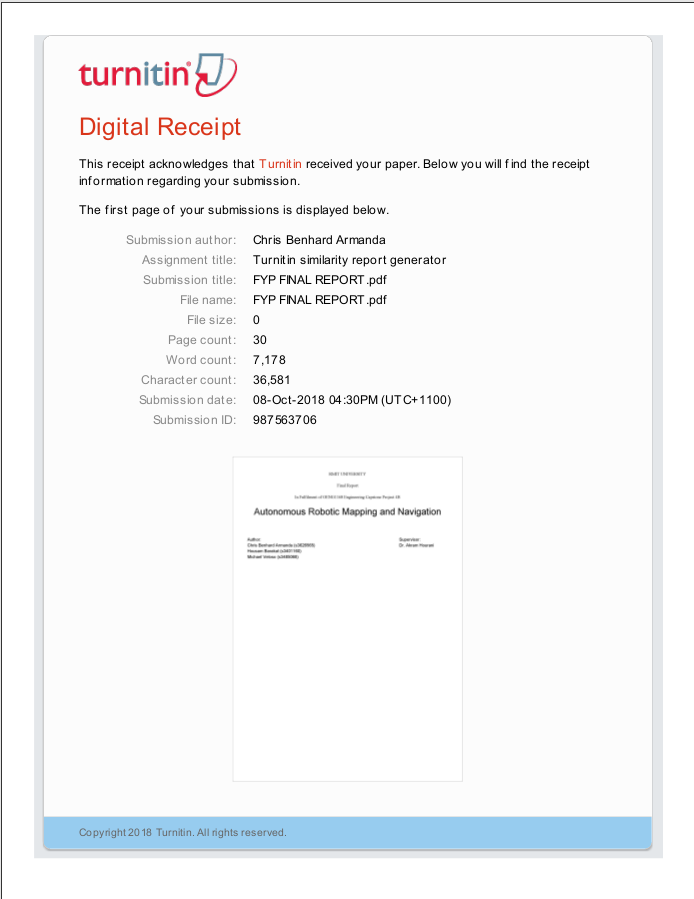
\includegraphics[scale=0.55]{turnitinreport.png}
\end{figure}
\end{document}
